\chapter{Rebuilding: A New Take on \Egraph Invariant Maintenance}
\label{sec:rebuild}
\label{sec:rebuilding}

% Rebuilding is a new, general perspective on \egraph invariant maintenance.
Traditionally~\cite{nelson, simplify},
  \egraphs maintain their data structure invariants
  after each operation.
We separate this invariant restoration into a procedure called \textit{rebuilding}.
This separation allows the client to
  choose when to enforce the \egraph invariants.
Performing a rebuild immediately after every operation replicates the
  traditional approach to invariant maintenance.
In contrast, rebuilding less frequently can amortize the cost of invariant
  maintenance, significantly improving performance.

In this section, we first describe how e-graphs have
  traditionally maintained invariants (\autoref{sec:upward}).
We then describe the rebuilding framework and how it captures a spectrum of
  invariant maintenance approaches, including the traditional one
  (\autoref{sec:rebuilding-detail}).
Using this flexibility, we then give a modified algorithm for equality
  saturation that enforces the \egraph invariants at only select points
  (\autoref{sec:rebuilding-eqsat}).
We finally demonstrate that this new approach offers an asymptotic speedup over
  traditional equality saturation (\autoref{sec:rebuild-eval}).

% Among \egg's optimizations (\autoref{sec:egg-efficient}),
%   strategically delayed rebuilding is perhaps the most important.
% \egg employed a m
% Delayed rebuilding amortizes the cost of invariant maintenance, significantly reducing work

% Rebuilding is a novel technique that lies at the heart of \egg's
%   modified equality saturation algorithm.
% This crucial technique allows equality saturation to specialize the \egraph to
%   its workload, yielding substantial performance improvements.
%   %from both an algorithmic and implementation
%   %perspective.

% Rebuilding gives the user (or algorithm) choice on when to restore the \egraph
%   invariants, which can have a large impact on performance .

% The key insight is that maintaining the \egraph invariants is expensive, and

% \autoref{fig:eq-sat-code} shows both the traditional and \egg's modified
%   equality saturation loop.
% The key distinction is \textit{when} the \egraph invariants of deduplication and
%   congruence are maintained.
% In traditional \egraphs, like with many data structures, invariants always
%   hold.
% In contrast, mutating an \egg \egraph may violate invariants, causing equalities
%   to be not ``seen'' when searching for patterns.
% \egg lets the user (or the algorithm) choose when to restore the invariants by
%   calling the \texttt{rebuild} method.
% Rebuilding leads to a lower amortized cost of maintaining the \egraph invariants.

\section{Upward Merging}
\label{sec:upward}

Both mutating operations on the \egraph
  (\texttt{add} and \texttt{merge}, \autoref{sec:interface})
  can break the \egraph invariants if not done carefully.
\Egraphs have traditionally used \textit{hashconsing} and
  \textit{upward merging} to maintain the congruence invariant.

The \texttt{add} operation relies on the hashcons invariant
  (Definition \ref{def:hash-inv})
  to quickly check whether the \enode $n$ to be added---or one congruent to it---is
  already present.
Without this check, \texttt{add} would create a new \eclass with $n$ in it
  even if some $n' \cong n$ was already in the \egraph,
  violating the congruence invariant.

The \texttt{merge} operation \eclasses can violate both \egraph invariants.
If $f(a, b)$ and $f(a, c)$ reside in two different \eclasses $x$ and $y$,
  merging $b$ and $c$ should also merge $x$ and $y$ to maintain the congruence invariant.
This can propagate further, requiring additional merges.

 % merging $x$ and $y$ could cause two other
 %  \enodes to become congruent and require merging their \eclasses.

\Egraphs maintain a \textit{parent list} for each \eclass
  to maintain congruence.
The parent list for \eclass $c$ holds all \enodes that have $c$ as a child.
When merging two \eclasses, \egraphs inspect these parent lists to find parents
  that are now congruent, recursively ``upward merging'' them if necessary.

The \texttt{merge} routine must also perform bookkeeping to preserve the
  hashcons invariant.
In particular, merging two \eclasses may change how parent \enodes of those
  \eclasses are canonicalized.
The \texttt{merge} operation must therefore
  remove, re-canonicalize, and replace those \enodes in the
  hashcons.
In existing \egraph implementations~\cite{herbie} used for equality saturation,
  maintaining the invariants while merging can take the vast majority of
  run time.

\section{Rebuilding in Detail}
\label{sec:rebuilding-detail}

\begin{figure}
  \begin{minipage}[t]{0.47\linewidth}
    \begin{lstlisting}[gobble=4, numbers=left, basicstyle=\scriptsize\ttfamily, escapechar=|, xleftmargin=13pt, numbersep=7pt]
    def add(enode):
      enode = self.canonicalize(enode)
      if enode in self.hashcons:
        return self.hashcons[enode]
      else:
        eclass_id = self.new_singleton_eclass(enode)
        for child in enode.children:
          child.parents.add(enode, eclass_id)
        self.hashcons[enode] = eclass_id
        return eclass_id

    def merge(id1, id2)
      if self.find(id1) == self.find(id2):
        return self.find(id1)
      new_id = self.union_find.union(id1, id2)
      # traditional egraph merge can be
      # emulated by calling rebuild right after
      # adding the eclass to the worklist
      self.worklist.add(new_id) |\label{line:worklist-add}|
      return new_id

    def canonicalize(enode) |\label{line:canon}|
      new_ch = [self.find(e) for e in enode.children]
      return mk_enode(enode.op, new_ch)

    def find(eclass_id):
      return self.union_find.find(eclass_id)
    \end{lstlisting}
  \end{minipage}
  \hfill
  \begin{minipage}[t]{0.45\linewidth}
    \begin{lstlisting}[gobble=4, numbers=left, firstnumber=27, basicstyle=\scriptsize\ttfamily, numbersep=7pt]
    def rebuild():
      while self.worklist.len() > 0:
        # empty the worklist into a local variable
        todo = take(self.worklist)
        # canonicalize and deduplicate the eclass refs
        # to save calls to repair
        todo = { self.find(eclass) for eclass in todo }
        for eclass in todo:
          self.repair(eclass)

    def repair(eclass):
      # update the hashcons so it always points
      # canonical enodes to canonical eclasses
      for (p_node, p_eclass) in eclass.parents:
        self.hashcons.remove(p_node)
        p_node = self.canonicalize(p_node)
        self.hashcons[p_node] = self.find(p_eclass)

      # deduplicate the parents, noting that equal
      # parents get merged and put on the worklist
      new_parents = {}
      for (p_node, p_eclass) in eclass.parents:
        p_node = self.canonicalize(p_node)
        if p_node in new_parents:
          self.merge(p_eclass, new_parents[p_node])
        new_parents[p_node] = self.find(p_eclass)
      eclass.parents = new_parents
    \end{lstlisting}
  \end{minipage}
  \caption{
    Pseudocode for the \texttt{add}, \texttt{merge}, \texttt{rebuild}, and
    supporting methods.
    In each method, \texttt{self} refers to the \egraph being modified.
  }
  \label{fig:rebuild-code}
\end{figure}

Traditionally, invariant restoration is part of the
  \texttt{merge} operation itself.
Rebuilding separates these concerns,
  reducing \texttt{merge}'s obligations
  and allowing for amortized invariant maintenance.
In the rebuilding paradigm,
  \texttt{merge} maintains a \textit{worklist} of \eclass ids that need to
  be ``upward merged'', i.e., \eclasses whose parents are possibly congruent but
  not yet in the same \eclass.
The \texttt{rebuild} operation processes this worklist, restoring the invariants
  of deduplication and congruence.
Rebuilding is similar to other approaches in how it restores congruence
  (see \nameref{sec:related} for comparison to \cite{downey-cse});
  but it uniquely allows the client to choose when to restore invariants in the
  context of a larger algorithm like equality saturation.

\autoref{fig:rebuild-code} shows pseudocode for the main \egraph operations and
  rebuilding.
Note that \texttt{add} and \texttt{canonicalize} are given for completeness, but
  they are unchanged from the traditional \egraph implementation.
The \texttt{merge} operation is similar, but it only adds the new \eclass to the
  worklist instead of immediately starting upward merging.
Adding a call to \texttt{rebuild} right after the addition to
  the worklist (\autoref{fig:rebuild-code} line \ref{line:worklist-add})
  would yield the traditional behavior of restoring the invariants immediately.

The \texttt{rebuild} method essentially calls \texttt{repair} on the \eclasses
  from the worklist until the worklist is empty.
Instead of directly manipulating the worklist, \egg's \texttt{rebuild} method
  first moves it into a local variable and deduplicates \eclasses
  up to equivalence.
Processing the worklist may \texttt{merge} \eclasses,
  so breaking the worklist into chunks ensures that \eclass ids made
  equivalent in the previous chunk are deduplicated in the subsequent chunk.

The actual work of \texttt{rebuild} occurs in the \texttt{repair} method.
\texttt{repair} examines an \eclass $c$ and first canonicalizes \enodes in the
  hashcons that have $c$ as a child.
Then it performs what is essentially one ``layer'' of upward
  merging:
if any of the parent \enodes have become congruent, then their
  \eclasses are merged and the result is added to the worklist.

Deduplicating the worklist, and thus reducing calls to \texttt{repair},
  is at the heart of why deferring rebuilding improves
  performance.
Intuitively, the upward merging process of rebuilding traces out a ``path'' of
  congruence through the \egraph.
When rebuilding happens immediately after \texttt{merge}
  (and therefore frequently), these paths can substantially overlap.
By deferring rebuilding, the chunk-and-deduplicate approach can coalesce the
overlapping parts of these paths, saving what would have been redundant work.
In our modified equality saturation algorithm (\autoref{sec:rebuilding-eqsat}),
  deferred rebuilding is responsible for a significant, asymptotic speedup
  (\autoref{sec:rebuild-eval}).

\subsection{Examples of Rebuilding}

Deferred rebuilding speeds up congruence maintenance by amortizing the work of
  maintaining the hashcons invariant.
Consider the following terms in an \egraph:
  $f_{1}(x), ..., f_{n}(x),\, y_{1}, ..., y_{n}$.
Let the workload be $\texttt{merge}(x, y_{1}), ..., \texttt{merge}(x, y_{n})$.
Each merge may change the canonical representation of the $f_{i}(x)$s,
  so the traditional invariant maintenance strategy
  could require $O(n^{2})$ hashcons updates.
With deferred rebuilding the \texttt{merges} happen before
  the hashcons invariant is restored,
  requiring no more than $O(n)$ hashcons updates.

Deferred rebuilding can also reduce the number of calls to \texttt{repair}.
Consider the following $w$ terms in an \egraph,
  each nested under $d$ function symbols:
  $$f_1 (f_2(\ldots f_d(x_1))), \quad\ldots,\quad f_1(f_2(\ldots f_d(x_w)))$$
Note that $w$ corresponds the width of this group of terms, and $d$ to the depth.
Let the workload be $w-1$ merges that merge all the $x$s together:
  for $i \in [2, w], \texttt{merge}(x_{1}, x_{i})$.

In the traditional upward merging paradigm
  where \texttt{rebuild} is called after every \texttt{merge},
  each $\texttt{merge}(x_i, x_j)$ will require $O(d)$ calls to \texttt{repair}
  to maintain congruence, one for each layer of $f_{i}$s.
Over the whole workload, this requires $O(wd)$ calls to \texttt{repair}.

With deferred rebuilding, however, the $w-1$ merges can all take place before
  congruence must be restored.
Suppose the $x$s are all merged into an \eclass $c_{x}$
When \texttt{rebuild} finally is called,
  the only element in the deduplicated worklist is $c_{x}$.
Calling \texttt{repair} on $c_{x}$ will merge the \eclasses of the $f_{d}$
  \enodes into an \eclass $c_{f_{d}}$,
  adding the \eclasses that contained those \enodes back to the worklist.
When the worklist is again deduplicated,
  $c_{f_{d}}$ will be the only element,
  and the process repeats.
Thus, the whole workload only incurs $O(d)$ calls to \texttt{repair},
  eliminating the factor corresponding to the width of this group of terms.
\autoref{fig:repair-plot} shows that the number calls to \texttt{repair} is
  correlated with time spent doing congruence maintenance.

\subsection{Proof of Congruence}

Intuitively, rebuilding is a delay of the upward merging process, allowing
  the user to choose when to restore the \egraph invariants.
They are substantially similar in structure, with a critical a difference in when
  the code is run.
Below we offer a proof demonstrating that rebuilding restores the
\egraph congruence invariant.

\begin{theorem}
  Rebuilding restores congruence and terminates.
\end{theorem}

\begin{proof}
  Since rebuilding only merges congruent nodes,
    the congruence closure $\cong^{*}$ is fixed even though $\equivnode$ changes.
  When $(\equivnode) = (\cong^*)$, congruence is restored.
  Note that both $\equivnode$ and $\cong^*$ are finite.
  We therefore show that rebuilding causes $\equivnode$ to approach $\cong^*$.
  We define the set of incongruent \enode pairs as $I = (\cong^*) \setminus (\equivnode)$;
  in other words,
    $(n_{1}, n_{2}) \in I$ if $n_{1} \cong^{*} n_{2}$
     but $n_{1} \not\equivnode n_{2}$.
%    have the same function symbol
%    and equivalent children, but are not yet in the same \eclass.

  Due to the additive nature of equality saturation, $\equivnode$ only increases
    and therefore $I$ is non-increasing.
  However, a call to \texttt{repair} inside the loop of \texttt{rebuild} does
    not necessarily shrink $I$.
  Some calls instead remove an element from the worklist but do not modify the
    \egraph at all.

  Let the set $W$ be the worklist of \eclasses to be processed by
    \texttt{repair};
  in \autoref{fig:rebuild-code}, $W$ corresponds to \texttt{self.worklist} plus
    the unprocessed portion of the \texttt{todo} local variable.
  We show that each call to \texttt{repair} decreases the tuple
    $(|I|, |W|)$ lexicographically until $(|I|, |W|) = (0, 0)$,
    and thus rebuilding terminates with $(\equivnode) = (\cong^*)$.

  % If $I$ is empty, then $E = C$ by the definition of $I$, and the \egraph is
  %   congruent.
  % We show that, after rebuilding, both $I$ and $W$ are empty.

  Given an \eclass $c$ from $W$, \texttt{repair} examines $c$'s parents
    for congruent \enodes that are not yet in the same \eclass:
  \begin{itemize}
    \item If at least one pair of $c$'s parents are congruent,
          rebuilding merges each pair $(p_{1}$, $p_{2})$,
          which adds to $W$ but makes $I$ smaller by definition.
    \item If no such congruent pairs are found, do nothing.
          Then, $|W|$ is decreased by 1 since $c$ came from the
          worklist and \texttt{repair} did not add anything back.
  \end{itemize}

  Since $(|I|, |W|)$ decreases lexicographically,
    $|W|$ eventually reaches $0$, so \texttt{rebuild} terminates.
  Note that $W$ contains precisely those \eclasses that need to be
    ``upward merged'' to check for congruent parents.
  So, when $W$ is empty,
    \texttt{rebuild} has effectively performed upward merging.
%    albeit at a different time.
  By~\cite[Chapter 7]{nelson}, $|I| = 0$.
%    and is correct as per Nelson's
%  We therefore defer to Nelson's correctness
%    proof of the traditional upward merging algorithm
%    (Chapter 7, \cite{nelson})
%    to show that $|W| = 0$ implies $|I| = 0$.
Therefore, when rebuilding terminates, congruence is restored.

%  The \texttt{rebuild} method calls \texttt{repair} until $W$ is empty, so it
%  terminates.
%  If an \eclass had potentially incongruent parents,
%    then the \eclass would be in $W$.
%  Thus, if $W$ is empty, then no \eclasses have parents with incongruent \enodes,
%    so $I$ is empty as well,
%    and congruence is restored.
\end{proof}

\section{Rebuilding and Equality Saturation}
\label{sec:rebuilding-eqsat}

Rebuilding offers the choice of when to enforce the \egraph invariants,
  potentially saving work if deferred thanks to the deduplication of the
  worklist.
The client is responsible for rebuilding at a time that
  maximizes performance without limiting the application.

\begin{figure}
  \begin{subfigure}[t]{0.47\linewidth}
    \begin{lstlisting}[language=Python, gobble=6, numbers=left, basicstyle=\scriptsize\ttfamily, xleftmargin=13pt, numbersep=7pt]
      def equality_saturation(expr, rewrites):
        egraph = initial_egraph(expr)

        while not egraph.is_saturated_or_timeout():


          # reading and writing is mixed
          for rw in rewrites:
            for (subst, eclass) in egraph.ematch(rw.lhs):

              # in traditional equality saturation,
              # matches can be applied right away
              # because invariants are always maintained
              eclass2 = egraph.add(rw.rhs.subst(subst))
              egraph.merge(eclass, eclass2)

              # restore the invariants after each merge
              egraph.rebuild()

        return egraph.extract_best()
    \end{lstlisting}
    \caption{
      Traditional equality saturation alternates between searching and applying
      rules, and the \egraph maintains its invariants throughout.
    }
    \label{fig:eq-sat-code1}
  \end{subfigure}
  \hfill
  \begin{subfigure}[t]{0.47\linewidth}
    \begin{lstlisting}[language=Python, gobble=6, basicstyle=\scriptsize\ttfamily, numbers=left, numbersep=5pt]
      def equality_saturation(expr, rewrites):
        egraph = initial_egraph(expr)

        while not egraph.is_saturated_or_timeout():
          matches = []

          # read-only phase, invariants are preserved
          for rw in rewrites:
            for (subst, eclass) in egraph.ematch(rw.lhs):
              matches.append((rw, subst, eclass))

          # write-only phase, temporarily break invariants
          for (rw, subst, eclass) in matches:
            eclass2 = egraph.add(rw.rhs.subst(subst))
            egraph.merge(eclass, eclass2)

          # restore the invariants once per iteration
          egraph.rebuild()

        return egraph.extract_best()
    \end{lstlisting}
    \caption{
      \egg splits equality saturation iterations into read and write phases.
      The \egraph invariants are not constantly maintained, but restored
      only at the end of each iteration by the \texttt{rebuild} method
      (\autoref{sec:rebuild}).
    }
    \label{fig:eq-sat-code2}
  \end{subfigure}

  \caption{
    Pseudocode for traditional and \egg's version of the equality saturation
    algorithm.
  }
  \label{fig:eq-sat-code}
\end{figure}

\egg provides a modified equality saturation algorithm to take advantage
  of rebuilding.
\autoref{fig:eq-sat-code} shows pseudocode for both traditional equality
  saturation and \egg's variant, which exhibits two key differences:
\begin{enumerate}
  \item Each iteration is split into a read phase, which searches for all the
        rewrite matches, and a write phase that applies those matches.\footnote
    {
      Although the original equality saturation paper~\cite{eqsat}
      does not have separate reading and writing phases,
      some \egraph implementations (like the one inside Z3~\cite{z3})
      do separate these phases as an implementation detail.
      Ours is the first algorithm to take advantage of this by deferring
      invariant maintenance.
    }
  \item Rebuilding occurs only once per iteration, at the end.
\end{enumerate}

\egg's separation of the read and write phases means that rewrites are truly
  unordered.
In traditional equality saturation, later rewrites in the given rewrite list are
  favored in the sense that they can ``see'' the results of earlier rewrites in
  the same iteration.
Therefore, the results depend on the order of the rewrite list
  if saturation is not reached (which is common on large rewrite lists or input
  expressions).
\egg's equality saturation algorithm is invariant to the order of the rewrite
  list.

Separating the read and write phases also allows \egg to safely defer rebuilding.
If rebuilding were deferred in the traditional equality saturation algorithm,
  rules later in the rewrite list would be searched against an \egraph with
  broken invariants.
Since congruence may not hold, there may be missing equivalences, resulting in
  missing matches.
These matches will be seen after the \texttt{rebuild} during the next iteration
  (if another iteration occurs), but the false reporting could impact metrics
  collection, rule scheduling,\footnotemark{} or saturation detection.
\footnotetext{
  An optimization introduced in \autoref{sec:rule-scheduling} that
  relies on an accurate count of how many times a rewrite was matched.
}

\section{Evaluating Rebuilding}
\label{sec:rebuild-eval}

To demonstrate that deferred rebuilding
  provides faster congruence closure than traditional upward merging,
  we modified \egg to call \texttt{rebuild} immediately after every \texttt{merge}.
This provides a one-to-one comparison of deferred rebuilding against the
  traditional approach, isolated
  from the many other factors that make \egg efficient: overall design
  and algorithmic differences, programming language performance, and other
  orthogonal performance improvements.

\begin{figure}
  \centering
  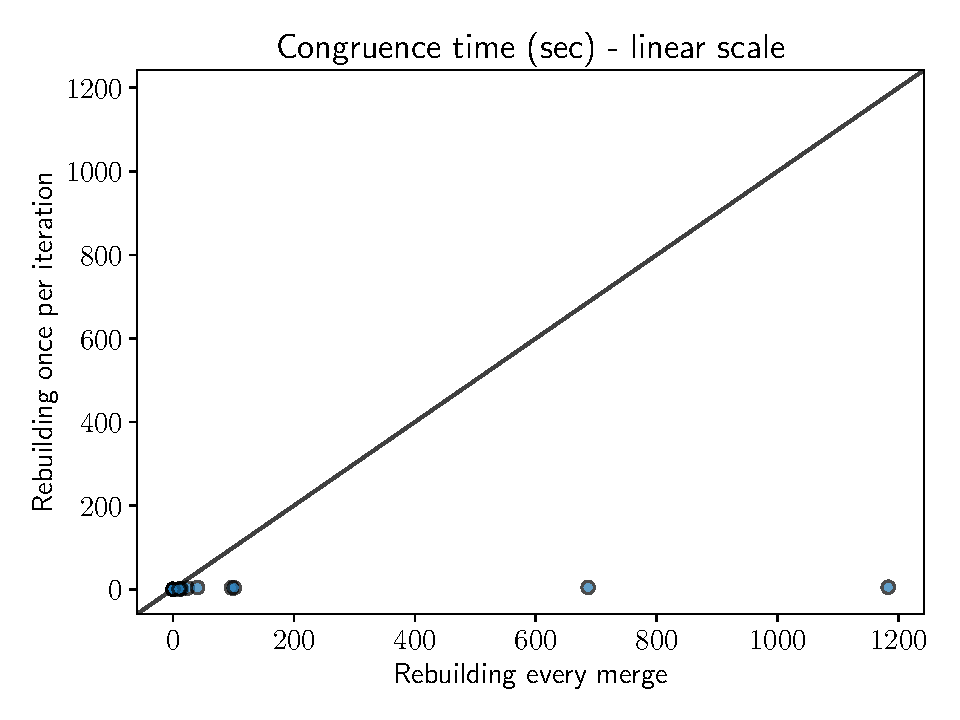
\includegraphics[width=0.7\linewidth]{speedup}
  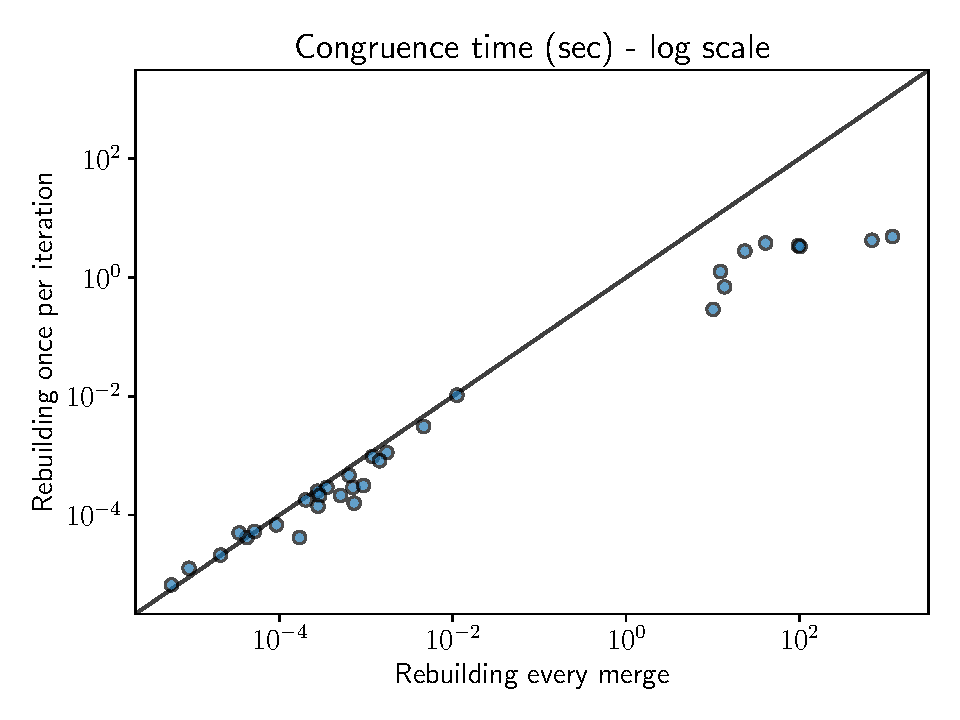
\includegraphics[width=0.7\linewidth]{speedup-log}
  \caption{
    Rebuilding once per iteration---as opposed to after every merge---significantly
      speeds up congruence maintenance.
    Both plots show the same data: one point for each of the \nEggTests tests.
    The diagonal line is $y=x$;
      points below the line mean deferring rebuilding is faster.
    In aggregate over all tests (using geometric mean),
      congruence is \CongrSpeedup faster, and
      equality saturation is \TotalSpeedup faster.
    The linear scale plot shows that deferred rebuilding is significantly faster.
    The log scale plot suggests the speedup is greater than some constant multiple;
      \autoref{fig:eval-iter} demonstrates this in greater detail.
  }\label{fig:eval}
\end{figure}

\begin{figure}
  \centering
  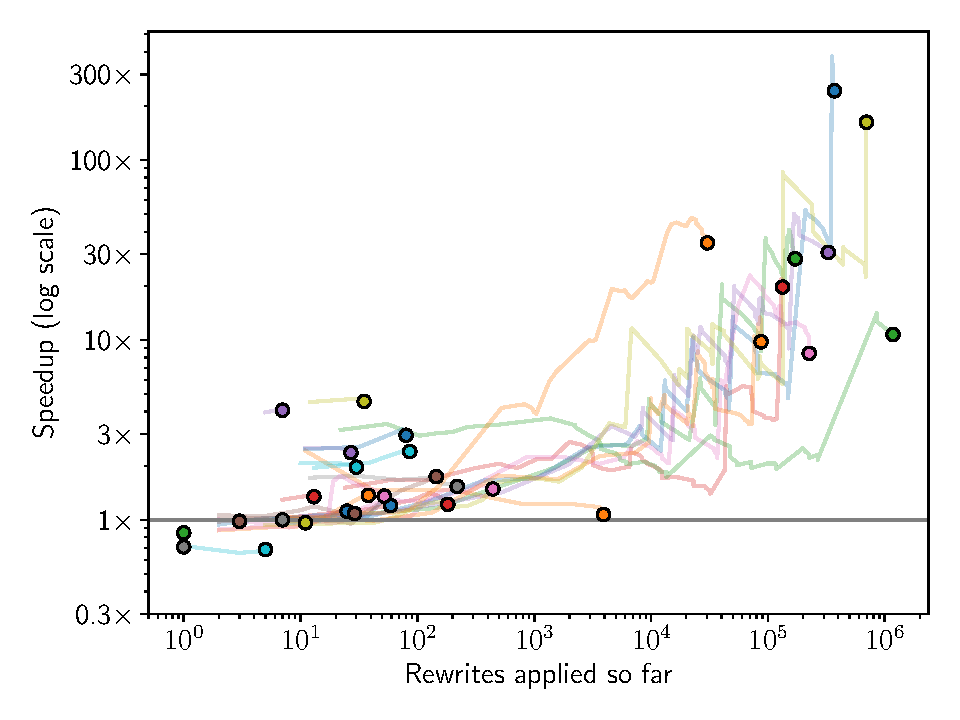
\includegraphics[width=0.6\linewidth]{speedup-iter}
  \caption{
    As more rewrites are applied, deferring rebuilding gives greater speedup.
    Each line represents a single test: each equality saturation iteration plots
      the cumulative rewrites applied so far against the multiplicative speedup
      of deferring rebuilding; the dot represents the end of that test.
    Both the test suite as a whole (the dots) and individual tests (the lines)
      demonstrate an asymptotic speedup that increases with
      the problem size.
  }
  \label{fig:eval-iter}
  \vspace{1em}

  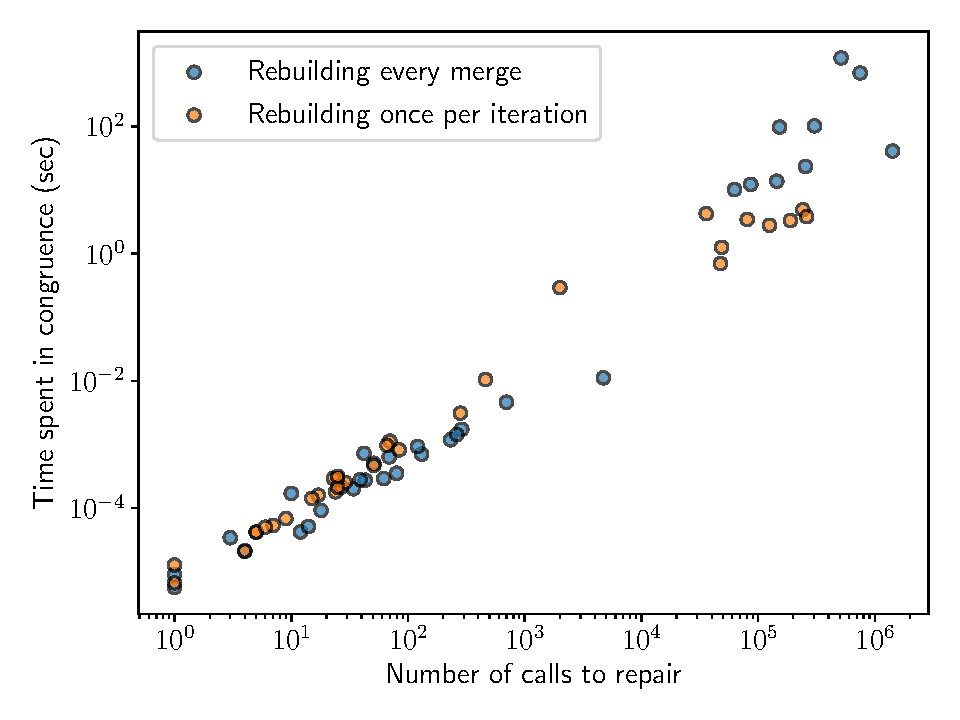
\includegraphics[width=0.6\linewidth]{repairs}
  \caption{
    The time spent in congruence maintenance correlates with the number of calls
    to the \texttt{repair} method.
    Spearman correlation yields $r=\RepairsR$ with a p-value of \RepairsP,
    indicating that the two quantities are indeed positively correlated.
  }
  \label{fig:repair-plot}
\end{figure}


We ran \egg's test suite using both rebuild strategies, measuring the time spent
  on congruence maintenance.
Each test consists of one run of \egg's equality saturation algorithm to optimize
  a given expression.
Of the \nEggTests total tests,
  \nEggTimeouts hit the iteration limit of 100 and the remainder saturated.
Note that both rebuilding strategies use \egg's phase-split equality saturation
  algorithm, and the resulting \egraphs are identical in all cases.
These experiments were performed on a 2020 Macbook Pro with a 2 GHz quad-core
  Intel Core i5 processor and 16GB of memory.

\autoref{fig:eval} shows our how rebuilding speeds up congruence maintenance.
Overall, our experiments show an aggregate \CongrSpeedup speedup on congruence
  closure and \TotalSpeedup speedup over the entire equality saturation
  algorithm.
\autoref{fig:eval-iter} shows this speedup is asymptotic;
  the multiplicative speedup increases as problem gets larger.

\egg's test suite consists of two main applications:
\texttt{math},
  a small computer algebra system capable of symbolic differentiation and
  integration; and
\texttt{lambda},
  a partial evaluator for the untyped lambda calculus using explicit
  substitution to handle variable binding (shown in \autoref{sec:impl}).
Both are typical \egg applications primarily driven by
  syntactic rewrites, with a few key uses of \egg's more complex features
  like \eclass analyses and dynamic/conditional rewrites.

\egg can be configured to capture various metrics about equality saturation as
  it runs, including the time spent in the read phase (searching for matches),
  the write phase (applying matches), and rebuilding.
In \autoref{fig:eval}, congruence time is measured as the time spent
  applying matches plus rebuilding.
Other parts of the equality saturation algorithm (creating the initial \egraph,
  extracting the final term) take negligible take compared to the equality
  saturation iterations.

Deferred rebuilding amortizes the examination of \eclasses
  for congruence maintenance;
  deduplicating the worklist reduces the number of calls to the \texttt{repair}.
\autoref{fig:repair-plot} shows that time spent in congruence is correlated with
  the number of calls to the \texttt{repair} methods.

The case study in \autoref{sec:herbie} provides a further evaluation of
  rebuilding. Rebuilding (and other \egg features) have also been implemented in
  a Racket-based \egraph, demonstrating that rebuilding is a conceptual advance
  that need not be tied to the \egg implementation.

%%% Local Variables:
%%% TeX-master: "../thesis"
%%% End:
